%  TEX program=xelatex

\documentclass[12p,UTF8]{article}
\setlength\paperheight{26cm}
\setlength\paperwidth{18.4cm}
\usepackage[fontset=windows,zihao={-4}]{ctex} % Chinese support, using Windows fonts
\usepackage{setspace} % 导入 setspace 宏包
\usepackage{graphicx} % Insert images
\usepackage{listings} % Print source code
\usepackage{color} % Color support
\usepackage{booktabs} % Professional table support
\usepackage{pdflscape} % Landscape pages support in PDF
\usepackage{hyperref} % Hypertext links support for cross-referencing
\usepackage{geometry} % Page layout customization
\usepackage{float}
\usepackage{subfigure}
\usepackage{fontspec} % 导入 fontspec 宏包，用于设置字体
% 
% \geometry{left = 8 cm, right=8cm , top = 3cm, bottom = 3cm}
% Customize hyperref format (it's set to no special format here)
\hypersetup{hidelinks}
% 设置全局页面边距
\geometry{left=3.17cm, right=3.17cm, top=2.54cm, bottom=2.54cm}
% 设置全局英文字体
\setmainfont{Times New Roman} % 你可以将 Times New Roman 替换为你想要的字体
% Declare directories to search for graphics files for graphicx
\graphicspath{{figures/}{logo/}}



% Define new command for title page
\newcommand{\reporttitle}[2]{
  \LARGE\textsf{#1}\quad\underline{\makebox[12em]{#2}}
}
\newcommand{\reportinfo}[2]{
  \large\makebox[4em]{\textsf{#1}}\quad\underline{\makebox[15em]{#2}}
}

% The document begins here
\begin{document}
\begin{spacing}{1.25} % 设置全局行距为1.25倍
  \begin{titlepage}
     \centering
     % \vspace*{0.2\fill}
     % \vspace*{-20pt}
     \includegraphics[width=\linewidth]{ahu1}\\[3cm] % Change the school logo here (See the logo/ directory) and adjust the height
     % \includegraphics[height=144pt]{pku-text-logo}\\[48pt] % Change the school logo here (See the logo/ directory) and adjust the height
     % {\huge\textsf{课\ 程\ 实\ 验\ 报\ 告}}\\[48pt]
     {\zihao{2} \heiti《数字电路与逻辑设计》\ 综\ 合\ 作\ 业}\\[4cm]
     % \reporttitle{实验名称}{立扫帚实验}\\[72pt]
     % \reportinfo{课程名称}{麻瓜研究}\\[8pt]
     \reportinfo{\zihao{-2}\songti 学\hspace{\fill}院}{\zihao{-2}\songti 电子信息工程学院}\\[10pt]
     \reportinfo{\zihao{-2}\songti 专\hspace{\fill}业}{\zihao{-2}\songti 电子信息工程专业}\\[8pt]
     \reportinfo{\zihao{-2}\songti 年\hspace{\fill}级}{\zihao{-2} \songti 23级}\\[8pt]
     \reportinfo{\zihao{-2}\songti 学\hspace{\fill}号}{\zihao{-2}\songti P12314101}\\[8pt]
     \reportinfo{\zihao{-2}\songti 姓\hspace{\fill}名}{\zihao{-2}\songti 章顺}\\
     \vspace*{\fill}
  \end{titlepage}
  % \newgeometry{left = 3.17cm, right = 3.17cm, top = 2.54cm , bottom=2.54cm}
  \tableofcontents
  \newpage
 \songti
  \section{问题描述与设计要求}
  \subsection{题目描述}
  试用74LS160设计一个三百六十五进制的计数器，并用数码管显示。要求各位间为十进制关系。
  允许附加必要的门电路。
  % \begin{enumerate}
  %   \item 学会寻找扫帚的重心，培养学生的耐心；
  %   \item 验证基本物理定律在霍格沃茨的有效性。
  % \end{enumerate}
  \subsection{设计要求}
  \begin{enumerate}
    \item 设计一个三百六十五进制的计数器；
    \item 用三片74LS160设计出一个模365的计数器；
    \item 使用数码管显示计数器的值；
    \item 将每一位上的二进制数转换为十进制且能够被数码管表示出来；
    \item 用单个数码管分别显示个十百位上的数字，个十百位分别用红蓝绿来表示；
    \item 各位间为十进制关系。
  \end{enumerate}
  \section{设计方案}
  \subsection{总体设计方案}
  根据题目要求电路设计将分为三大部分，第一部分时序产生，第二部分为模365的分频
  器设计，该部分为设计的核心部分，第三部分为数码管显示部分。\\[4cm]
  % Insert an image, with placement specifier htbp
  \begin{figure}[htbp]
    \centering
    
\includegraphics[width=0.5\textwidth]{alldesign}
    \caption{总设计原理框图}
    \label{alldesign}
  \end{figure}

  在第一部分的设计中应保证时序的稳定可靠。在第二部分的设计中考虑到设计的简单性
  同时方便与数码管连接选择以模10计数器为基本单元进行扩展，同时由365
  可计算得出至少需要三片模10计数器。在第三部分的设计中每一个计数器连
  接一个译码器便可实现数码管的显示。

  \begin{figure}[htbp]
    \centering
    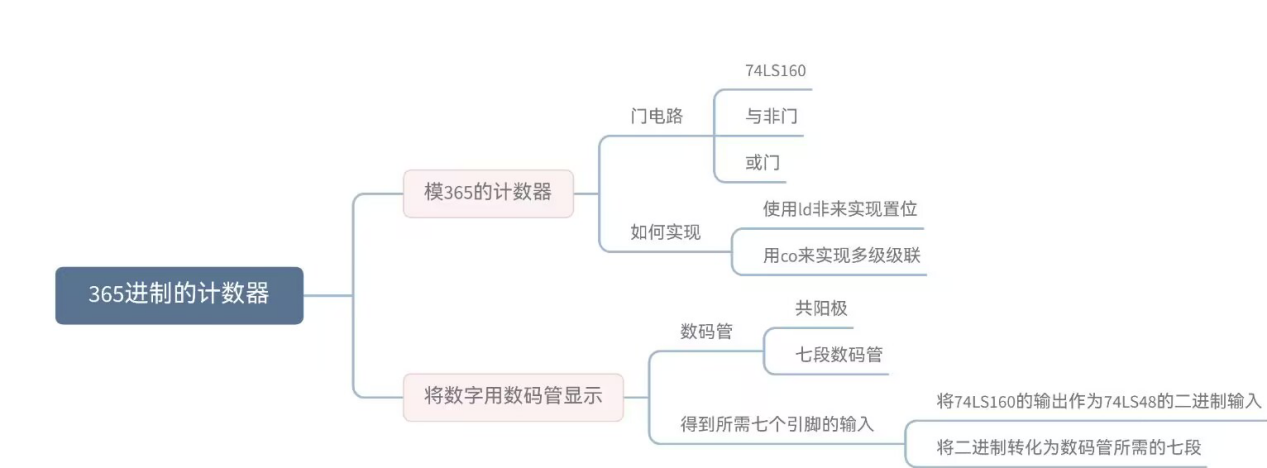
\includegraphics[width=0.8\textwidth]{swdt}
    \caption{设计过程思维导图}
    \label{swdt}
  \end{figure}
  % 实验具体要求如下：
  % \begin{enumerate}
  %   \item 扫帚必须能够单独站立，不可以借助其它外力；
  %   \item 实验过程中不得使用咒语，尤其是不得使用永久粘贴咒将扫帚粘在地上。
  % \end{enumerate}
  \subsection{脉冲发生器的选择}
  \subsubsection{555定器}
  555定时器是由模拟和数字电路相混合构成的集成电路。由于电路中使用了三个5kΩ
  的电阻，故取名为555电路。555电路只要外接少量阻容元器件，就可以组成单稳态
  触发器，多谐振荡器，多种波形发生器等。电路结构简单，性能可靠，使用方便，应
  用范围很广泛。555电路的内部结构及外围电路如图所示：

  \begin{figure}[H]
    \centering  %图片全局居中
    \subfigure[555内部结构]{
    \label{555in}
    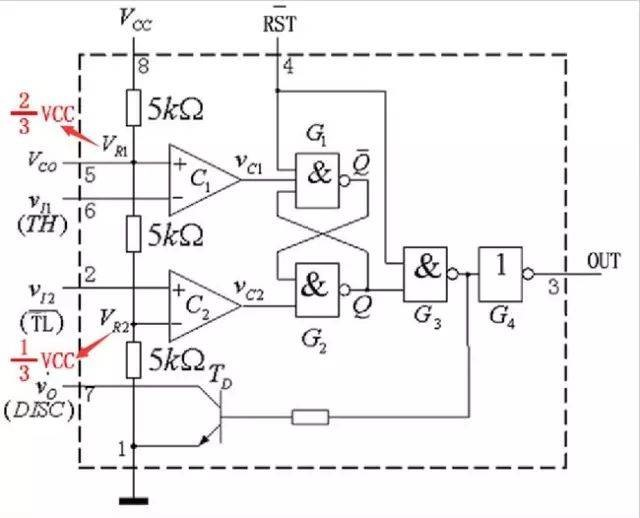
\includegraphics[width=0.45\textwidth]{555in}}\subfigure[555外围电路]{
    \label{555out}
    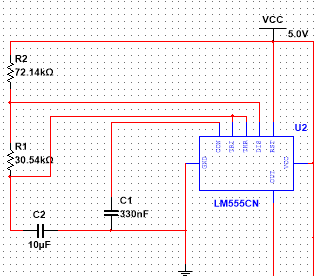
\includegraphics[width=0.45\textwidth]{555out}}
    \caption{555电路的内部结构及外围电路如图所示}
    \label{555}
  \end{figure}
    
  缺点：电路连接起来比较复杂，而且要求较多，接口也比较复杂。

  \subsubsection{DIGITAL\_CLOCK}
  DIGITAL\_CLOCK是一个生成周期性数字信号的组件。它可以作为数字组件的刺激源。
  你也可以使用时钟电压和时钟电流组件提供刺激。然而，DIGITAL\_CLOCK更有效率，
  因为它的模型中不包括模数转换和数模转换桥。它可以用于产生稳定的高频脉冲信号作
  为时间基准，经分频器输出标准的秒脉冲。提供了一种简单有效的方法来生成二号控制数
  字信号。

  \subsubsection{CLOCK\_CURRENT}
  CLOCK\_CURRENT是一个用于生成周期性电流信号的组件。这个组件可以作为电流源，
  为电路提供周期性的电流刺激。它的工作原理类似于DIGITAL\_CLOCK，但是输出的是
  电流信号，而不是电压信号。在电路设计和仿真中，CLOCK\_CURRENT可以用于模拟各
  种需要周期性电流输入的场景。例如，在一些电源电路、放大器电路或者电磁场模拟中
  ，CLOCK\_CURRENT可以作为输入源，提供稳定的周期性电流。
  \begin{figure}[H]
    \centering  %图片全局居中
    \subfigure[DIGITAL\_CLOCK]{
    \label{digitalclock}
    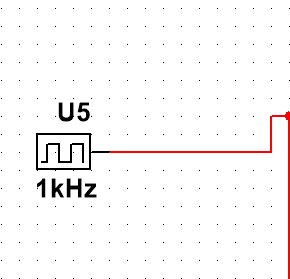
\includegraphics[width=0.45\textwidth]{digitalclock}}\subfigure[CLOCK\_CURRENT]{
    \label{clockcurrent}
    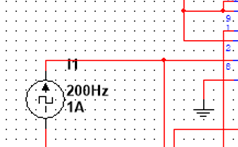
\includegraphics[width=0.45\textwidth]{clockcurrent.png}}
    \caption{Multisim中的脉冲发生器}
    \label{CLOCK}
  \end{figure}

  上述三个脉冲发生器都能实现相应的结果，此时考虑到电路的简便性，
  以及易实现的需求，因此，决定选择DIGITAL\_CLOCK作为最终的脉冲发生器。
  \subsection{模365电路}
  \subsubsection{74LS160的介绍}
  74LS160是可预置十进计数器，由四个D型触发器和若干个门电路构成，内部有超前进位，
  具有计数、置数、禁止、直接（异步）清零等功能。对所有触发器同时加上时钟，使得当计
  数使能输入和内部门发出指令时输出变化彼此协调一致而实现同步工作。这种工作方式消除
  了非同步（脉冲时钟）计数器中常有的输出计数尖峰。缓冲时钟输入将在时钟输入上升沿触发
  四个触发器。这种计数器是可全编程的，即输出可预置到任何电平。当预置是同步时，在置
  数输入上将建立一低电平，禁止计数，并在下一个时钟之后不管使能输入是何电平，输出都
  与建立数据一致。清除是异步的（直接清零），不管时钟输入、置数输入、使能输入为何电平，
  清除输入端的低电平把所有四个触发器的输出直接置为低电平。超前进位电路无须另加门，
  即可级联出n位同步应用的计数器。它是借助于两个计数使能输入和一个动态进位输出来实现的。
  两个计数使能输入（ENP和 ENT）计数时必须是高电平，且输入ENT必须正反馈，以便使能动态
  进位输出。因而被使能的动态进位输出将产生一个高电平输出脉冲，其宽度近似等于QA 输出高
  电平。此高电平溢出进位脉冲可用来使能其后的各个串联级。使能ENP和 ENT输入的跳变不受
  时钟输入的影响。电路有全独立的时钟电路。改变工作模式的控制输入（使能ENP、ENT或清零）
  纵使发生变化，直到时钟发生为止，都没有什么影响。计数器的功能（不管使能、不使能、置数
  或计数）完全由稳态建立时间和保持时间所要求的条件来决定。
  \begin{figure}[H]
    \centering  %图片全局居中
    \subfigure[74ls160ic]{
    \label{74ls160ic}
    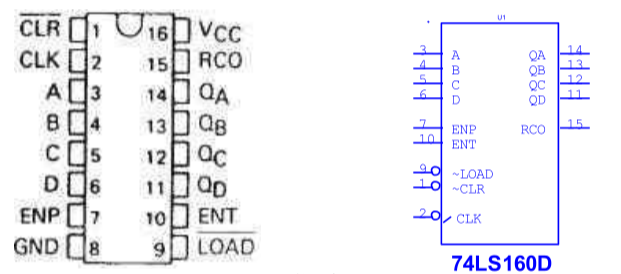
\includegraphics[width=0.45\textwidth]{74ls160ic.png}}
    \subfigure[真值表]{
    \label{74ls160zzb}
    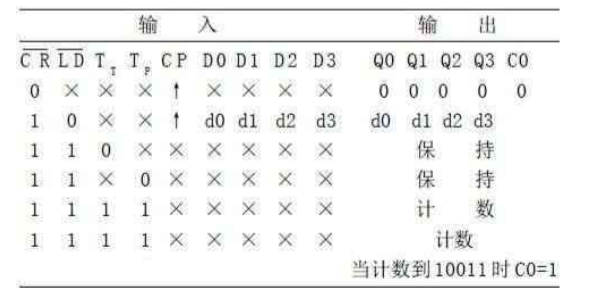
\includegraphics[width=0.45\textwidth]{74ls160zzb.png}}
    \caption{74ls160}
    \label{74ls60}
  \end{figure}

  \subsubsection{模365电路的构成}
  为了实现模365计数器的功能，采用了三片74LS160芯片，通过CO来控制下一级芯片的启动，
  通过三个芯片上对应的Q来实现置位功能，相关电路图如下：

  如图所示，计数器以QA1，QC1,QB2,QC2,QA3,QC3并在一起作为置位端,为了使电路更加
  简洁，所以采用了三个且非加上一个或门来实现置位。计数初值DCBA都为0000，当QA1，Q
  C1,QB2,QC2,QA3,QC3都为1时发出置位信号进行重新置数。因此，其实现了0和365两种不
  同状态的循环输出，从而能够实现一个模365的计数器。
  
  \begin{figure}[H]
    \centering
    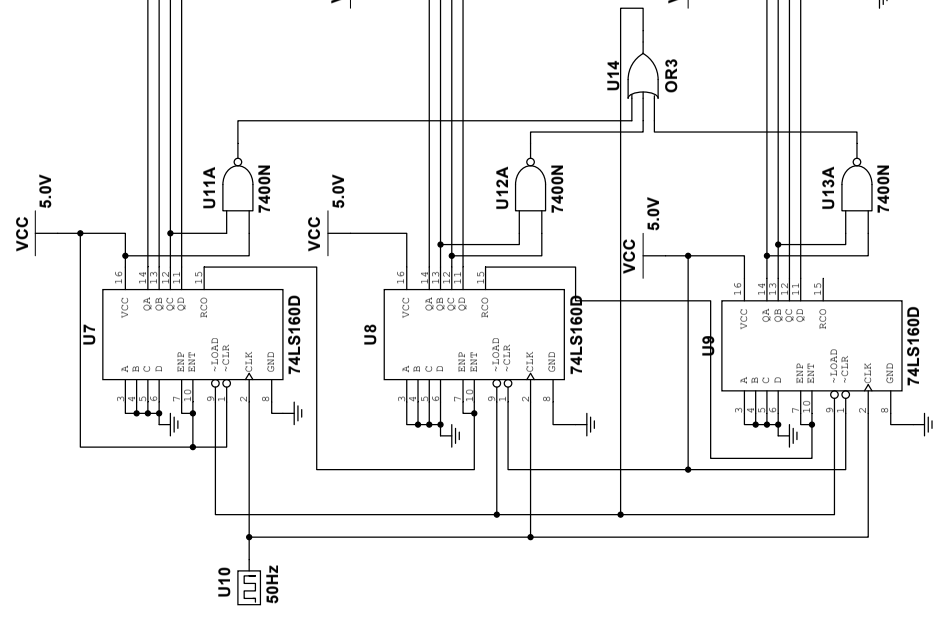
\includegraphics[width=0.8\textwidth]{m365.png}
    \caption{模365电路图}
    \label{m365}
  \end{figure}

  \subsection{数码管显示部分}
  \subsubsection{74LS48D介绍}
  74LS48是BCD至七段解码器，用于显示以二进制编码的十进制格式解码的数字。7 
  段是一种基于 7 个 LED 的小型设备，用于表示从 0 到 9 的单个数值。每个 
  7 段有七个输入引脚，用于点亮七个段中的单个 LED。每次制作单个数字时，
  某些特定引脚应该有电源输入。

  \subsubsection{工作原理}
  在 IC 74LS48 中，输出取决于输入。主要输入引脚有四个，有助于在特定输入
  数据上生成固定输出状态。在4位二进制数字中，十进制的0用0000表示，十进制的
  9用1001表示，并且从1到8的所有值也都有固定的4位二进制代码。当IC上有0到9的
  输入时，输出值将根据共阴极7段。这是因为 IC 是为执行该功能而设计的。如果使
  用7段IC，我们需要根据给定的电路连接7段IC。

  \begin{figure}[H]
    \centering
    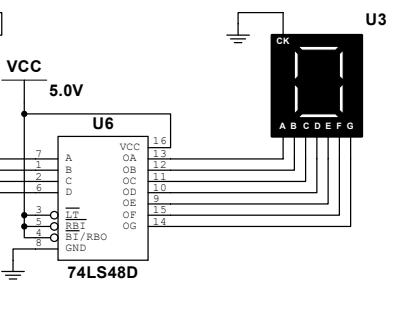
\includegraphics[width=0.7\textwidth]{smg.png}
    \caption{数码管显示部分}
    \label{smg}
  \end{figure}

  \section{总电路图及仿真结果}
  \begin{figure}[H]
    \centering
    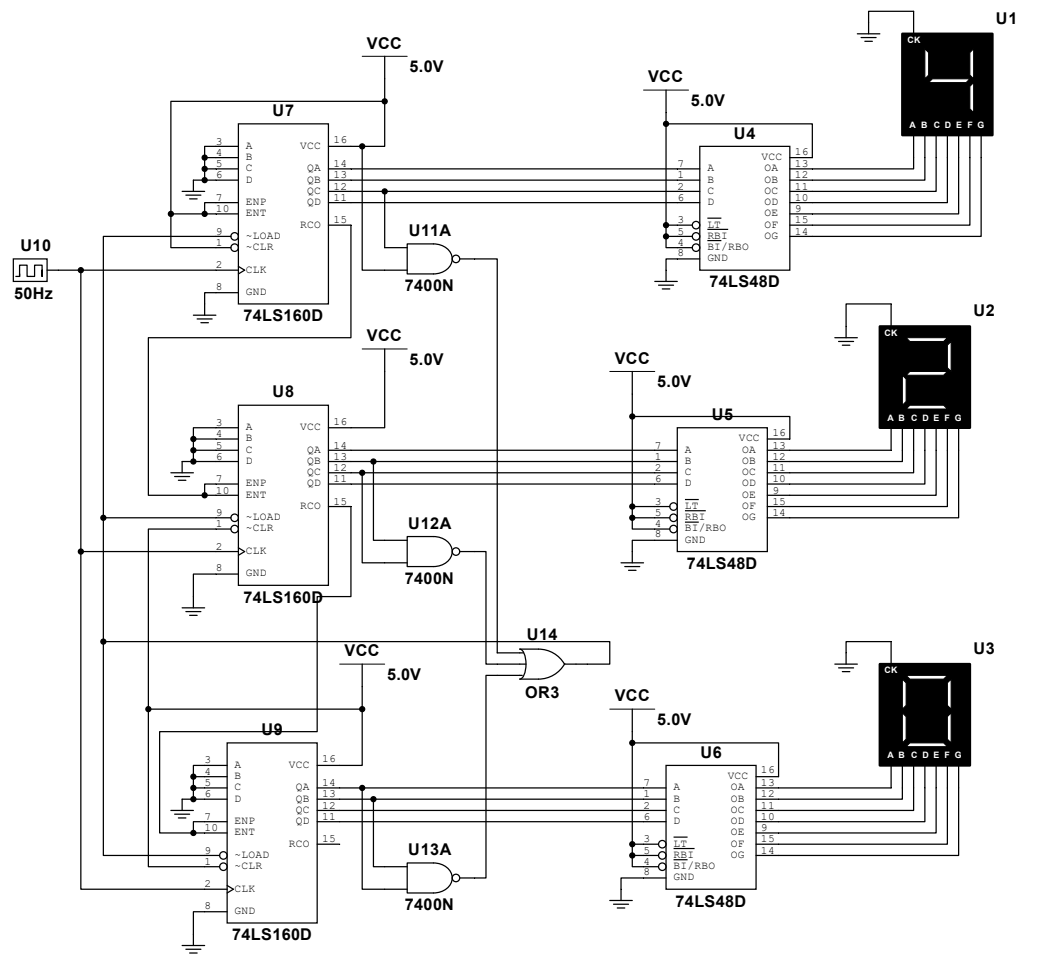
\includegraphics[width=0.7\textwidth]{all.png}
    \caption{总电路图}
    \label{all}
  \end{figure}
  
  \begin{figure}[H]
    \centering  %图片全局居中
    \subfigure[仿真结果1]{
    \label{rs1}
    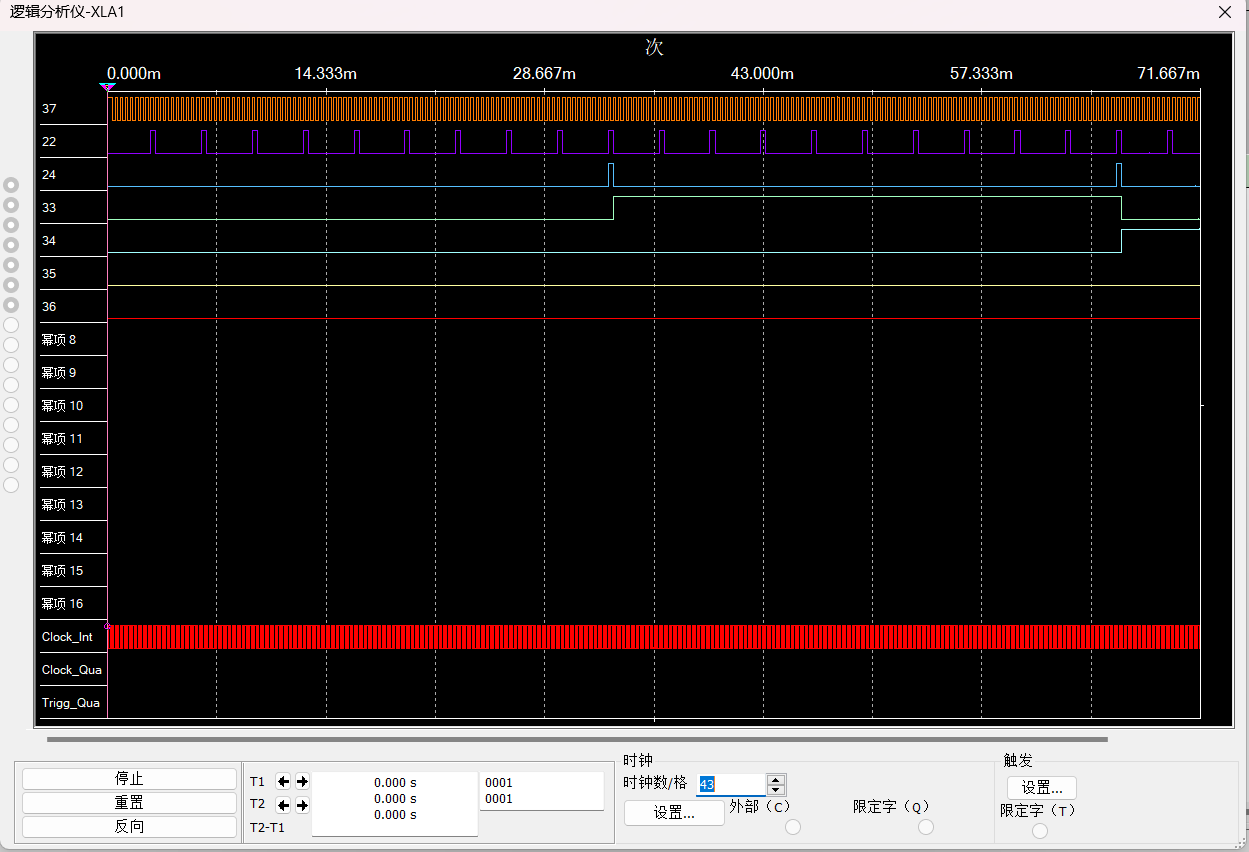
\includegraphics[width=0.48\textwidth]{rs1.png}}
    \subfigure[仿真结果2]{
    \label{rs2}
    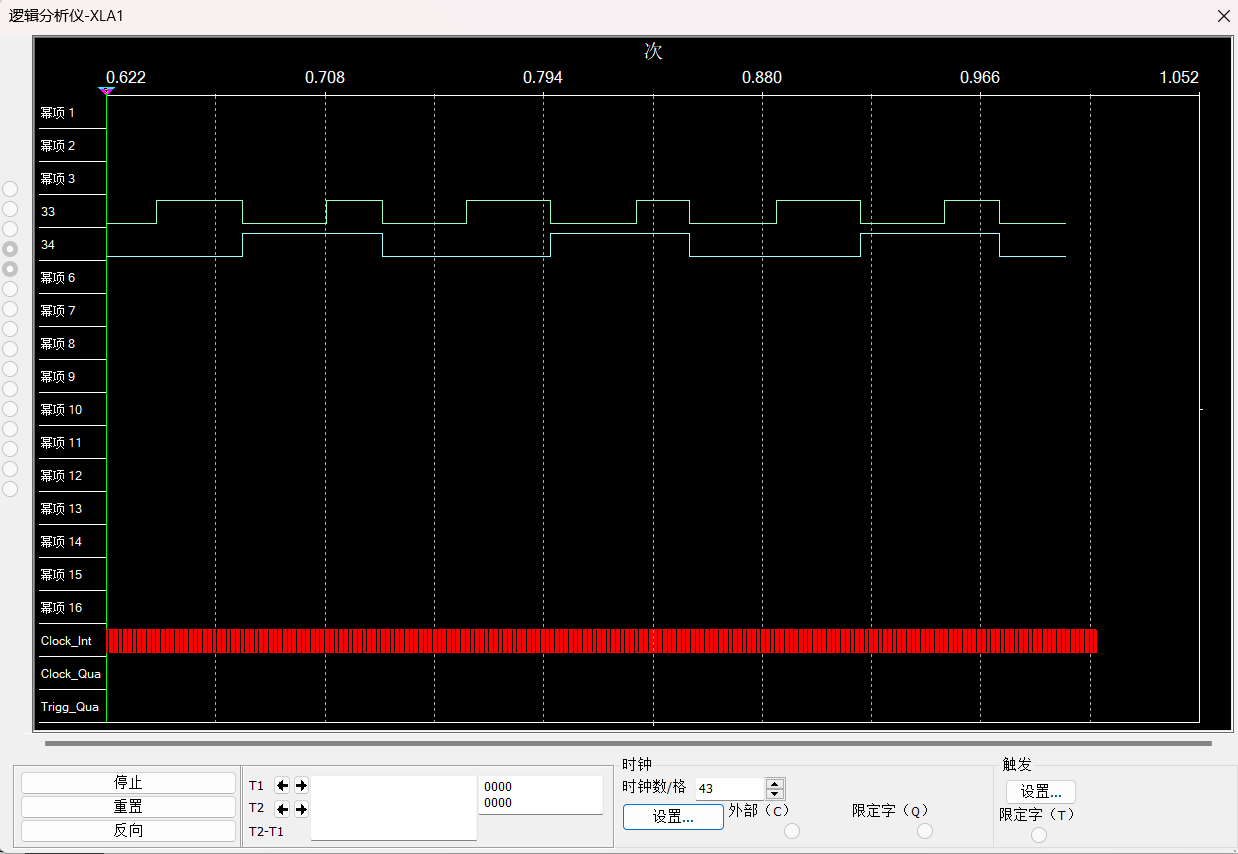
\includegraphics[width=0.48\textwidth]{rs2.png}}
    \subfigure[仿真结果3]{
    \label{rs3}
    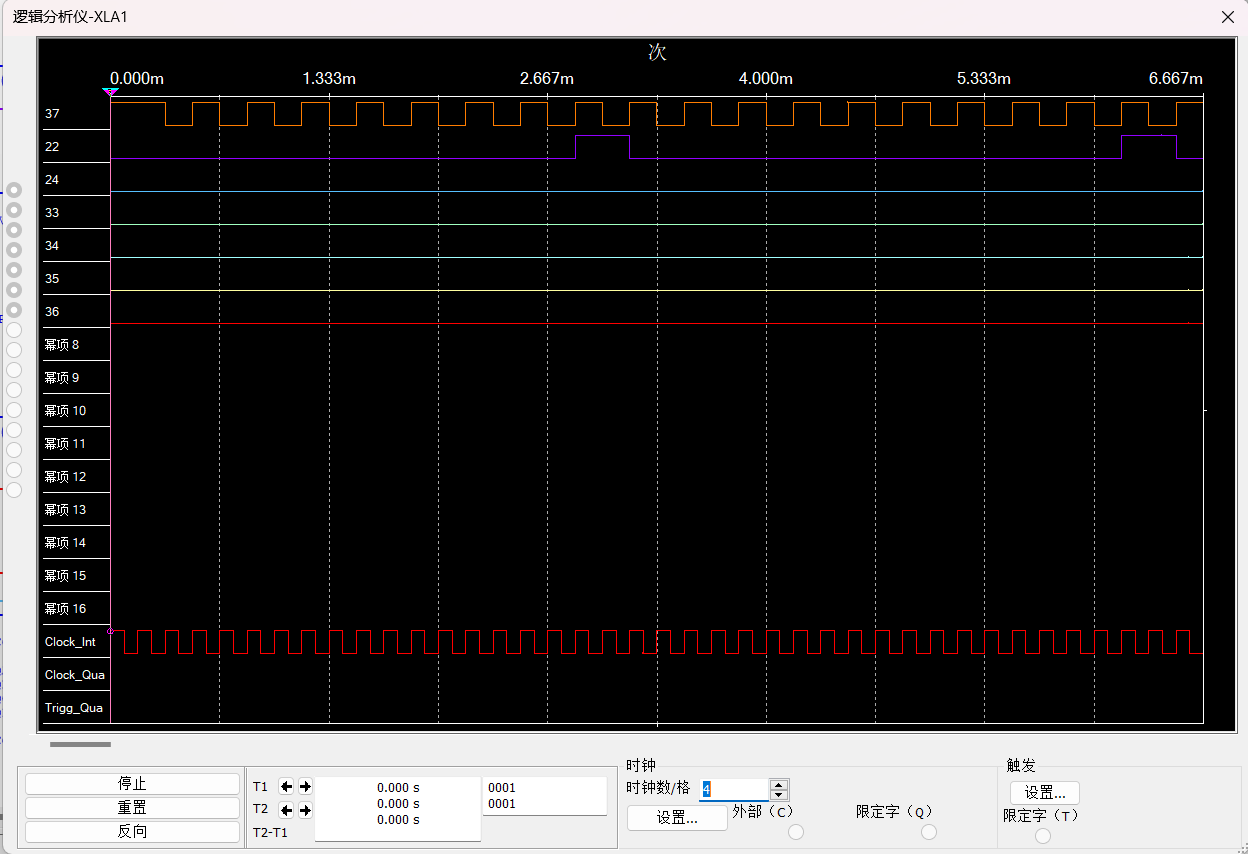
\includegraphics[width=0.6\textwidth]{rs3.png}}
    \caption{仿真结果}
    \label{rs}
  \end{figure}

  \section{实验总结}
  在本次课程设计中，我学习了如何利用数字集成电路芯片、数码管、逻辑门等元件，
  设计一个365进制的计数器，并用数码管显示其计数结果。我通过以下几个步骤完成了
  设计任务：



  \begin{enumerate}
    \item 分析设计要求，确定计数器的功能、性能、结构和原理。
    \item 选择合适的数字集成电路芯片，如74LS160十进制计
          数器、74LS48数码管译码器、与非门和或门等。
    \item 设计计数器的电路图，包括时序产生、模365计数器、数码管显示等部分。
    \item 利用Multisim软件进行电路仿真和调试，验证电路的正确性和稳定性。
    \item 撰写设计报告，总结设计过程和结果，提出改进建议和展望。
  \end{enumerate}

  通过本次课程设计，我不仅掌握了数字集成电路芯片的基本性质和功能，还了解了数
  码管的工作原理和显示方法，其次我也遇到了相关的问题。比如刚开始不知道在仿真中CLR要接1，以及刚开始没有检查
  电路，将或门用成了非门，导致结果一直无法出现，其中还遇到了数码管闪烁，接触不良的
  现象等，这些都通过自己摸索总结，查资料，分析电路在后面得到了解决。

  \section{实验感悟}
  我认为这个设计任务是一个有趣而富有挑战性的问题，它考验了我的数字电路知识和创造力。
  我在设计过程中遇到了一些困难，例如如何实现计数器的进位和清零逻辑，
  如何利用逻辑门实现高位灭零功能，如何使用Multisim软件进行电路仿真和调试等。
  我通过查阅资料，参考其他人的设计方案，反复修改和优化我的电路图，最终完成了这个设计任务。

  我从这个设计任务中学到了很多东西，不仅是关于数字电路的理论和实践，
  还有关于设计思维和方法的技巧。我学会了如何分析设计要求，选择合适的方案，
  设计电路图，仿真和调试电路，撰写设计报告等。我还学会了如何运用集成电路芯片，
  数码管，逻辑门等元件，设计出一个符合要求的计数器。并且，在自己动手的过程中我还加
  深了对于数电知识的理解深度。我觉得这些知识和技能对我今后的学习都有很大的帮助。

  我也意识到了自己的不足之处，例如我对数字电路的基础知识还不够扎实，我对电路设计软
  件的使用还不够熟练，我对电路的性能和效率的评估还不够全面，我对设计报告的格式和内
  容的规范还不够清晰等。我希望在今后的学习中，我能够不断提高自己的水平，掌握更多的
  知识和技能，设计出更好的电路。



\end{spacing}
\end{document}


 % \section{实验过程}
  % \subsection{扫帚的选择}
  % 不同的扫帚参数各异，这里列出了部分扫帚的参数，请见表 \ref{broomsticks}。

  % % Insert a three-line table
  % \begin{table}[htbp]
  %   \centering
  %   \begin{tabular}{cccc}
  %     \toprule
  %     序号 & 名称 & 上市时间 & 最高时速 \\
  %     \midrule
  %     1 & 彗星290 & 1995年 & 60\,mph \\
  %     2 & 光轮1000 & 1967年 & 100\,mph \\
  %     3 & 光轮2001 & 1992年 & >\,100\,mph \\
  %     4 & 火弩箭 & 1993年 & 150\,mph \\
  %     \bottomrule
  %   \end{tabular}
  %   \caption{部分扫帚的参数对比}
  %   \label{broomsticks}
  % \end{table}


  % Insert source code
  % \lstinputlisting[style=cpp-style]{random.cpp}

  % Insert an image in a separate landscape page
  % \begin{landscape}
  %   \begin{figure}
  %     \centering
  %     
\includegraphics[width=\linewidth]{Nimbus2001}
  %     \caption{光轮2001扫帚}
  %     \label{Nimbus2001}
  %   \end{figure}
  % \end{landscape}

  % \begin{figure}
  %   % \centering
  %   
\includegraphics[width=\linewidth]{Nimbus2001}
  %   \caption{光轮2001扫帚}
  %   \label{Nimbus2001}
  % \end{figure}

  % \subsection{扫帚起竖}
  % 光轮 2001 扫帚如图 \ref{Nimbus2001} 所示，与麻瓜使用的扫帚相比，有以下区别：
  % \begin{enumerate}
  %   \item 扫帚末端较尖，同时在各个方向上都不是平面；
  %   \item 扫帚柄有一定弯曲，重心不易估计。
  % \end{enumerate}